
\clearpage
\section{Procurement Function}

The procurement function supports the user when it comes to managing small or big tendering procedures. The procurements module is comprised of

\begin{itemize}
\item the procurement creation,
\item the tender inspection,
\item the award procedure,
\item the award approval and
\item the contracts.
\end{itemize}

\vspace{\baselineskip}

In addition, it is possible to illustrate different work-flows:

\begin{itemize}
\item Procurements with direct award (with one or more bidders).
\item Procurements by invitation or open procedure.
\end{itemize}

\vspace{\baselineskip}

Since the work-flows of a procurement vary from company to company or even from project to project, this module (Procurement function) is custom made and documented for the procedures of a client. In this chapter, possible procurement processes are carried out and documented by way of example.

\vspace{\baselineskip}

\textbf{Introduction :}

In order to facilitate the navigation, procurements (invitations / calls for tender), tenders, and contracts are numbered. When creating these elements, you will be required to establish the connection (which tender concerns which procurement, which contract concerns which tender). The numbering is accordingly composed:

\vspace{\baselineskip}

Procurement n. 28 with corresponding tender n. 45 will appear in the list of tenders with the number 28.45. If contract n. 31 is added in connection to these documents, it will appear in the list of contracts with the number 28.45.31. The numbers are automatically set by CUBE PA.

\subsection{Work-flow for procurement with direct award}

This work-flow can be used for procedures with one or more bidders. \\
The work-flow is comprised of the following steps:

\begin{enumerate}
\item Creating documents for the call for tender
\item Initializing the procurement
\item Uploading documents for the call for tender
\item Sending the call for tender
\item Receiving and uploading tenders
\item Establishing tender inspection logs and sending them to the decision-making body
\item Approval of the procedure by a position of higher order
\item Establishing a contract.
\end{enumerate}

Statuses are used for progress monitoring when working with procurements. The statuses in the following table describe a typical project progress.

\vspace{\baselineskip}

\begin{tabular}{|p{5cm}|p{9.5cm}|}    % p{9.5cm} l} %{cl}  % {|m{5.316cm}|m{9.586cm}|}
\hline
\textbf{Status} & \textbf{Who sets the status under which conditions} \\
\hline
Call for tender creation & This status is set automatically when a procurement is initialized. \\
\hline
Approved by X & You set this status once X has reviewed the call for tender. \\
\hline
Call for tender sent to invitees & You set this status when you have sent the call for tender to the tenderers (for direct award
and invitation procedures). \\
\hline
Tender inspection & You set this status once you've entered a tender. \\
\hline
Tender with X & You set this status once you've sent this tender along with its tender inspection log to X. \\
\hline
Decision position of higher order & You set this status once you've sent this tender along with its tender inspection log to X, and that it's stated in the tender inspection log, that for example a decision from a political authority is required. \\
\hline
Award made & X sets this status once the responsible project manager or a higher authority have approved the award. \\
\hline
Contract issued & X sets this status once they have sent the unsigned contract to the tenderer. \\
\hline
Signature X / Dispatch & X sets this status once they have sent the contract, signed by the tenderer, to the awarded tenderer and the general manager. \\
\hline
Procurement completed & You set this status once you've uploaded the contract. \\
\hline
\end{tabular}

\vspace{\baselineskip}

The statuses in the following table describe a discontinuation or a halt in project progress :

\vspace{\baselineskip}

\begin{tabular}{|p{5cm}|p{9.5cm}|}    % p{9.5cm} l} %{cl}  % {|m{5.316cm}|m{9.586cm}|}
\hline
\textbf{Status} & \textbf{Who sets the status under which conditions} \\
\hline
Tender(s) refused / archived & You set this status when project management decides that this tender will no longer be followed. Project management can also set this status. \\
\hline
Tender sent back for revision & You set this status when project management decided that this tender should be sent back for revision. Project management can also set this status. \\
\hline
\end{tabular}

\subsubsection{Step 1: Establishing documents for the call for tender}

You can create the documents for the call for tender using Excel and Word, or other suitable programs.

\subsubsection{Step 2: Initializing the procurement}

\begin{wrapfigure}[3]{l}{6.5cm}   % [x] Wie manche Zeile soll sich um die Grafik "brechen"
  \vspace{-35pt}      % Grundwert war 20; mit 30 schön oben beim Text ausgerichtet
  \begin{center}
    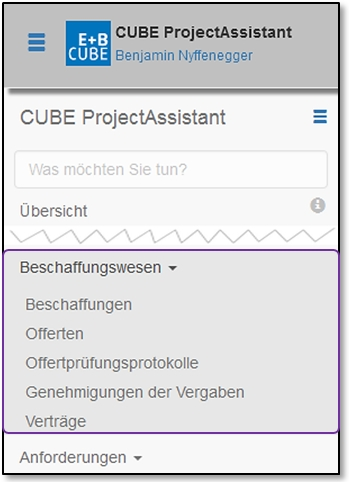
\includegraphics[width=1\linewidth]{../chapters/07_Beschaffungswesen/pictures/7-1-2_Menu_Beschaffungswesen.jpg}
  \end{center}
  \vspace{-20pt}
  \caption{Using the procurement function}
  \vspace{-10pt}
\end{wrapfigure}

In the menu on the left, select the menu item 'Procurement Function' and the sub-item 'Procurements'. 

\vspace{5cm}

The list of procurements is shown.

\vspace{2cm}

\begin{figure}[H]
\center{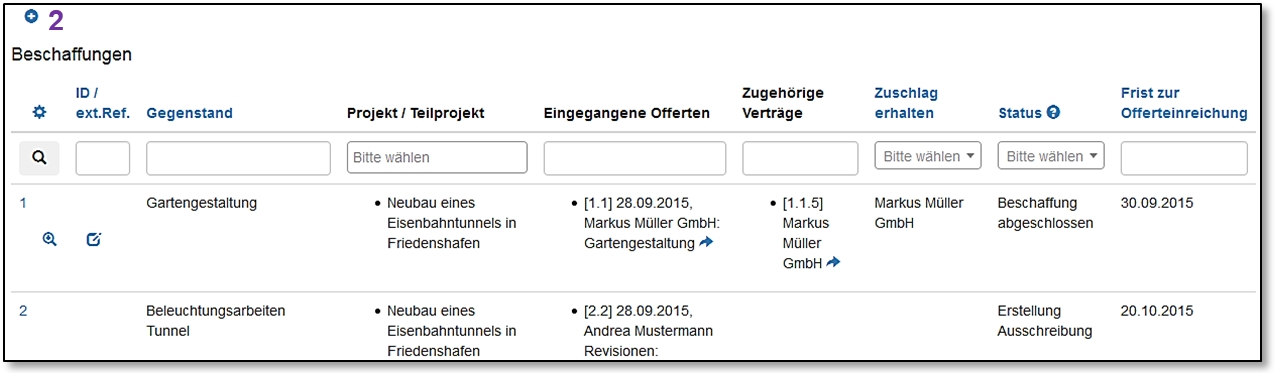
\includegraphics[width=1\linewidth]{../chapters/07_Beschaffungswesen/pictures/7-1-2_Beschaffung_Uebersicht.jpg}}
\caption{Procurements overview}
% \label{fig:speciation}
\end{figure}

% Problem

% \pagebreak
Click on the plus symbol 
\includegraphics[height=12pt]{/Icons/Plussymbol.jpg} \col{(2)} at the top left. The form for creating a new procurement appears:

\vspace{\baselineskip}

Mandatory fields are marked with an asterisk *.

\begin{figure}[H]
\center{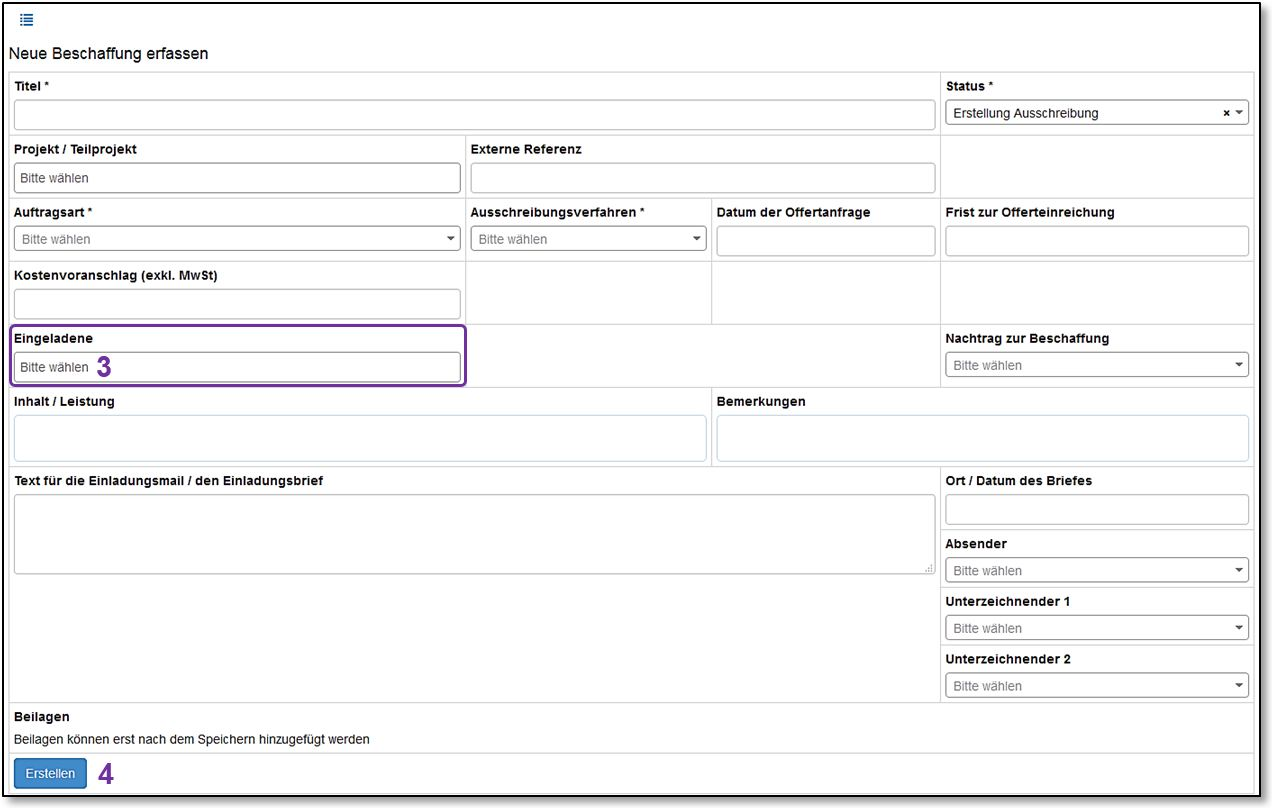
\includegraphics[width=1\linewidth]{712_BeschaffungErfassen.jpg}}
\caption{Creating a new procurement}
% \label{fig:speciation}
\end{figure}

First check if the drop-down menu of the 'Invitees' field \col{(3)} contains the company to which you want to send a call for tender. If this is not the case, switch to the 'Configuration' module in the menu on the left (see Chapter \ref{bkm:Ref434830029}) and enter the company there (Administrative rights are required for this step. Contact your CUBE PA spokesperson). If the company is in the list, select it. You can then fill out the rest of the fields:

\vspace{\baselineskip}

\begin{compactitem}
\item
Subject: Free text, short and concise.
\item
Status: Is automatically set to 'Call for tender creation' and should remain so.
\item
Project / Subproject: Select one or more corresponding project(s) / Subproject(s).
\item
External Reference: This field is only needed for retroactive logging of procurements that were in another list > not to be used.
\item
Type of order: Choose between construction contract and services contract.
\item
Tendering Procedure: Select 'Direct award'.
\item
Date of Publication: Choose the date of the tender invitation from the calendar.
\item
Deadline of Submission: Choose the deadline for receiving the tender form the calendar.
\item
Cost estimate: If there's a cost estimate, you can enter it here. You can only use numbers and one point. You will later have a direct comparison between the estimate and the tender offer.
\item
Supplementary Budget for Procurement: In case this procurement is a supplementary one for another procurement (this can be a reason why only one tenderer is written down), you can select the other procurement from the list.
\item
Content: Short description in free text of the expected services from the awarded tender, not more than 2 to 3 lines.
\item
Remarks: You can enter specific conditions for this procurement here, in later steps as well.
\item
Text for invitation mail / letter: Type the whole text of the tender invitation e-mail / letter here, with the exception of the place, time, and address. With this content, you can later generate a complete e-mail or letter invitation.
\item
If you want to send the tender invitation as a hard copy, fill out the fields 'Date, Place of Issue' (free text), 'Sender' (Drop-down selection list for the company sending the letter), 'Signature 1' (Selection list) and 'Signature 2' (Selection list). 'Signature 1' is higher in the hierarchy in case two signatures are needed.
\end{compactitem}

\vspace{\baselineskip}

Now click on the 'Create' \col{(4)}, and you can now add
attachments:

\begin{figure}[H]
\center{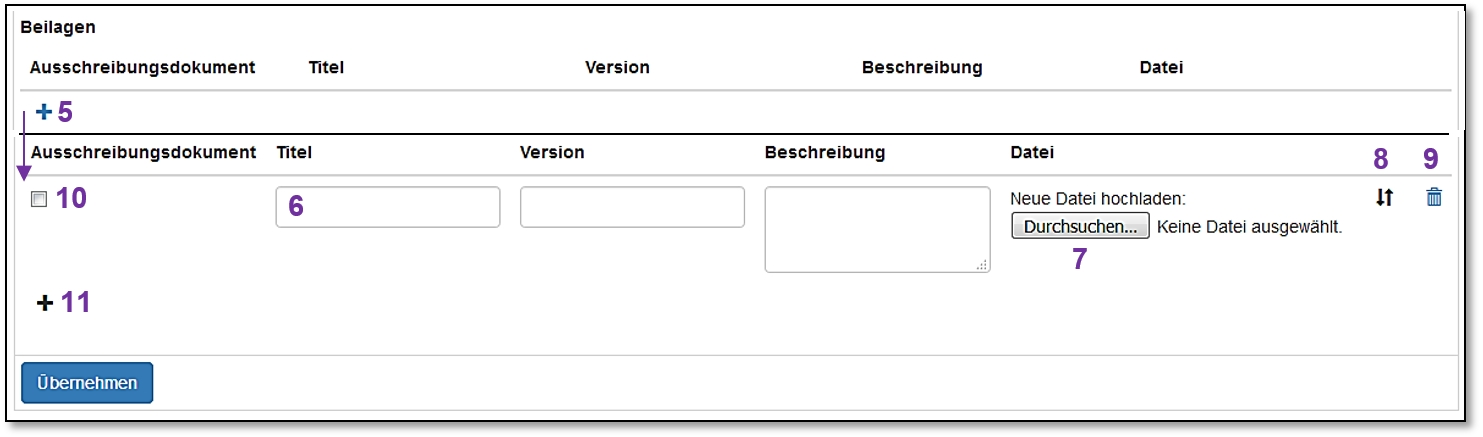
\includegraphics[width=1\linewidth]{../chapters/07_Beschaffungswesen/pictures/7-1-2_Beschaffung_Beilagen_hochladen.jpg}}
\caption{Uploading attachments to procurements}
% \label{fig:speciation}
\end{figure}

To add an attachment, click on the plus sign 
\includegraphics[height=12pt]{/Icons/Pluszeichen.jpg} \col{(5)}. You can now fill out the fields \col{(6)} and click 'Browse' \col{(7)} to upload a file. The arrows 
\includegraphics[height=12pt]{/Icons/VertPfeile.jpg} \col{(8)} allow you to change the order of an entry when you have multiple attachments (Drag and drop the arrows to place the attachment at the desired position). The garbage bin symbol 
\includegraphics[height=12pt]{/Icons/Muelltonne.jpg} \col{(9)} allows you to delete an attachment.
If you need to download the uploaded documents with the call for tender (to send the tender invitation for example), check the 'Tender Document' check-box \col{(10)}. You can add more documents using the plus symbol \includegraphics[height=12pt]{/Icons/pluszeichen.jpg} \col{(5)}. Close the process by clicking on 'Update'.

\vspace{\baselineskip}

You can now proceed immediately with step 3 or continue at a later time.

\vspace{\baselineskip}

\textbf{Intermediate step: Retroactively modifying a procurement or continuing with a procurement after an
an interruption}

\vspace{\baselineskip}

It is not necessary to proceed from step 2 to step 4 directly immediately one after the other. It is also possible to retroactively modify data after finishing a step. You can always access these steps from the procurements list. In the menu on the left, choose the 'Procurement Function' item and the 'Procurements' sub-item. The procurements list appears.

\vspace{\baselineskip}

You can visually search for a procurement within the list or filter the list to find it. To browse through the pages of the list, scroll down then use the pagination buttons to go to the next or previous page or a specific page number.

\begin{center}

\includegraphics[height=12pt]{/Icons/SeitenBlaettern.jpg}
\end{center}

To filter the list, use the search fields in the top row of the table. In the 'ID / Ext. Ref.' field, you can enter a number. The ID is the number given by CUBE PA. The 'Title' field is a free text field. The 'Project / Subproject' field is a drop-down selection list. The 'Deadline of Submission' field has a calendar selection. Once you've filled the filter fields, click on the magnifying glass symbol 
\includegraphics[height=12pt]{/Icons/Lupe_kl.jpg} \col{(1)} on the right, and the filtered list appears.

\begin{figure}[H]
\center{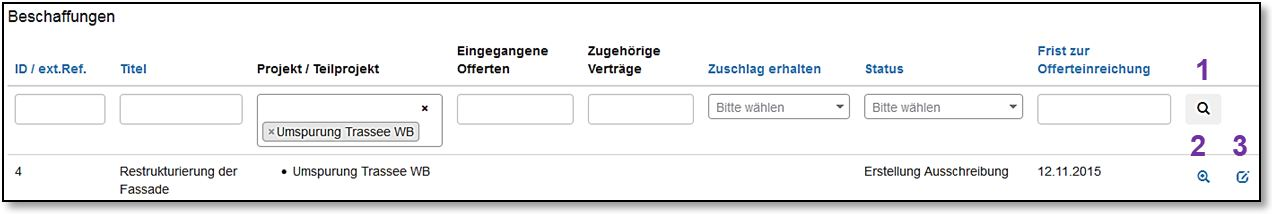
\includegraphics[width=1\linewidth]{712_BeschaffungFiltern.jpg}}
\caption{Filtering the procurements list}
% \label{fig:speciation}
\end{figure}

If you only wish to view an entry, without making any changes, click on the blue magnifying glass symbol 
\includegraphics[height=12pt]{/Icons/Lupe.jpg} \col{(2)}. The procurement entry will be opened. If you click on the pen symbol 
\includegraphics[height=12pt]{/Icons/Bearbeiten.jpg} \col{(3)}, the form for editing the procurement entry will be opened.\textcolor{red}{ } Now you can either correct existing data or continue to the next steps.

\subsubsection{Step 3: Uploading documents for the call for tender}

In this step you can add your previously prepared documents for the call for tender as attachments in CUBE PA.

\vspace{\baselineskip}

To add an attachment, click on the plus symbol 
\includegraphics[height=12pt]{/Icons/Pluszeichen.jpg} \col{(1)}. The following fields appear:

\begin{figure}[H]
\center{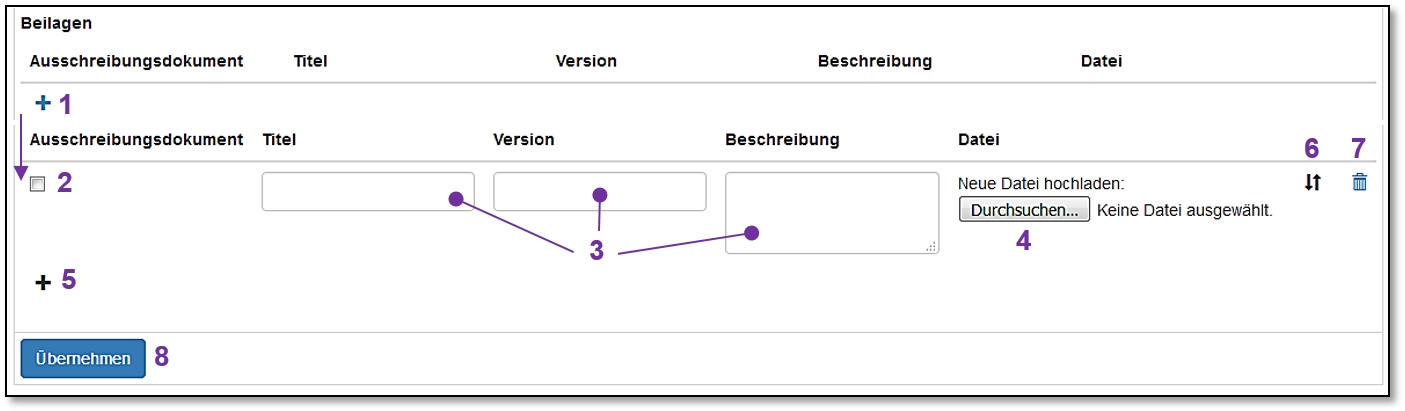
\includegraphics[width=1\linewidth]{../chapters/07_Beschaffungswesen/pictures/7-1-3_OffertanfrageHochladen.jpg}}
\caption{Uploading an attachment for the call for tender}
% \label{fig:speciation}
\end{figure}

\begin{itemize}
\item If the attachment is a tender document (to be sent with the call for tender), check the box 'Tender Document' \col{(2)}.
\item Title, version, and description are free text fields \col{(3)}. In many cases it's enough to just fill the title field.
\item Click on 'Browse' \col{(4)} to select a file to be uploaded. In case
you have selected the wrong file, simply upload a new one.
\item The plus symbol \includegraphics[height=12pt]{/Icons/pluszeichen.jpg} \col{(5)} enables you to add additional attachments.
\item You can change the order of the attachments by dragging and dropping the symbol with vertical arrows 
\includegraphics[height=12pt]{/Icons/VertPfeile.jpg} \col{(6)}.
\item Click on the garbage bin symbol 
\includegraphics[height=12pt]{/Icons/Muelltonne.jpg} \col{(7)} to delete an attachment.
\item After you've uploaded the files and filled out their details (title, etc.), click on 'Update' \col{(8)} to save.
\end{itemize}

\textbf{Hint :} The file name of the the uploaded attachment is automatically set in the 'Title' field. You can then change the title.

\subsubsection{Step 4: Sending the call for tender}

At the top left of the procurement edit form, click on the paper plane symbol 
\includegraphics[height=12pt]{/Icons/Versandsymbol.jpg}. The page for sending appears. At the left, the invited tenderers are listed \col{(1)}, in the middle, you can click again on the paper plane symbol 
\includegraphics[height=12pt]{/Icons/Versandsymbol.jpg} \col{(2)} to generate an e-mail, and on the left you can click on the envelope symbol 
\includegraphics[height=12pt]{/Icons/Briefsymbol.jpg} \col{(3)} to generate a PDF-file of the letter that you can then print out.

\begin{figure}[H]
\center{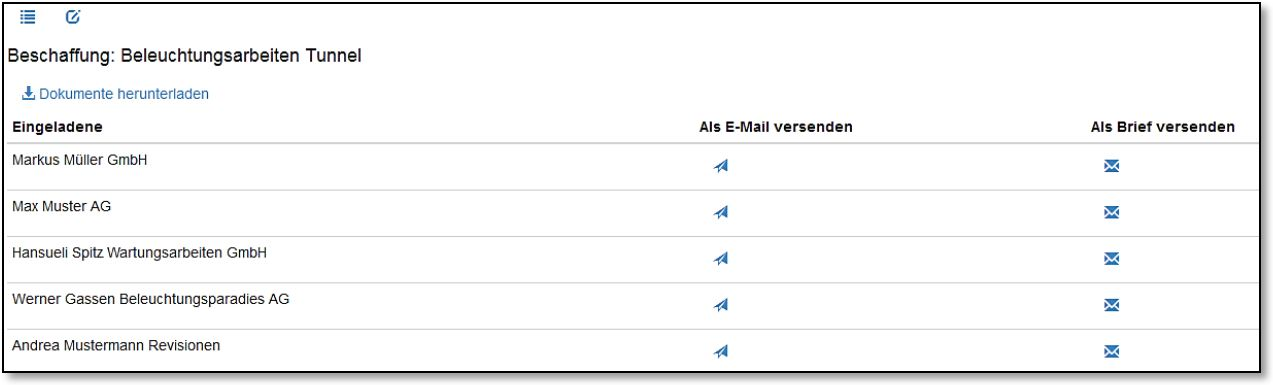
\includegraphics[width=1\linewidth]{714_BeschaffungVersand.jpg}}
\caption{Sending the call for tender}
% \label{fig:speciation}
\end{figure}

If there are attachments, the 'Download documents' button \col{(4)} appears at the top of the table. Downloading the tender documents is only needed if you want to print out the attachments to send them along with the invitation letter.

\vspace{\baselineskip}

When you click on the paper plane symbol 
\includegraphics[height=12pt]{/Icons/Versandsymbol.jpg}, the generated e-mail is opened in your e-mail programme. Check if the recipients, text, and signature are correct and complete the e-mail if required. The attachments are not enclosed to the e-mail, but a download link through which the recipients can directly download the attachments from the CUBE PA database is included. This way, problems that can occur when sending large files by e-mail are avoided.

\begin{wrapfigure}[7]{r}{6cm}
\vspace{-15pt}
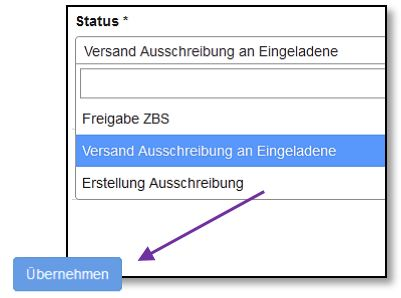
\includegraphics[height=50mm]{714_BeschaffungEingeladene.jpg}
% \caption{Status ändern}
\end{wrapfigure}

Go back to the list of procurements (menu on the left, menu item 'Procurement Function', sub-item 'Procurements'), open the procurement in edit mode by clicking on the pen symbol 
\includegraphics[height=12pt]{/Icons/Bearbeiten.jpg} and set its status to 'Call for tender sent to invitees'. Then click on 'Update'.

\vspace{\baselineskip}

\subsubsection{Step 5: Receiving and uploading tenders}

In the menu on the left, select the menu item 'Procurement Function' and then the sub-item 'Tenders'. The list of tenders appears.

\begin{figure}[H]
\center{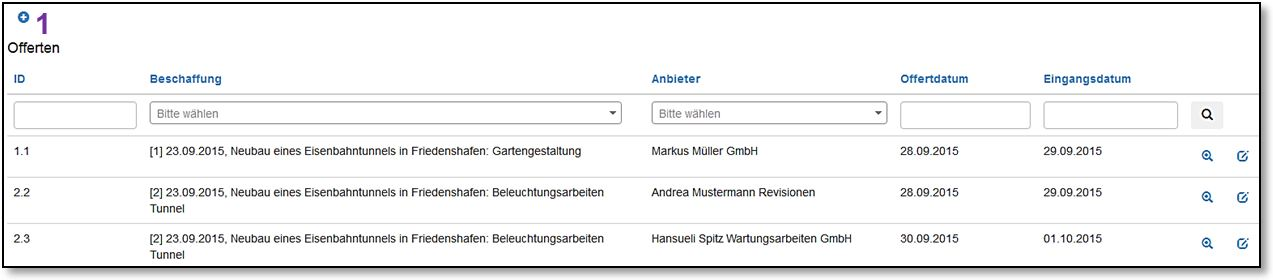
\includegraphics[width=1\linewidth]{715_OfferteUebersicht.jpg}}
\caption{Overview of the tenders}
% \label{fig:speciation}
\end{figure}

Click on the plus symbol 
\includegraphics[height=12pt]{/Icons/Plussymbol.jpg} \col{(1)} at the top left. The form for adding new tenders appears.

\begin{figure}[H]
\center{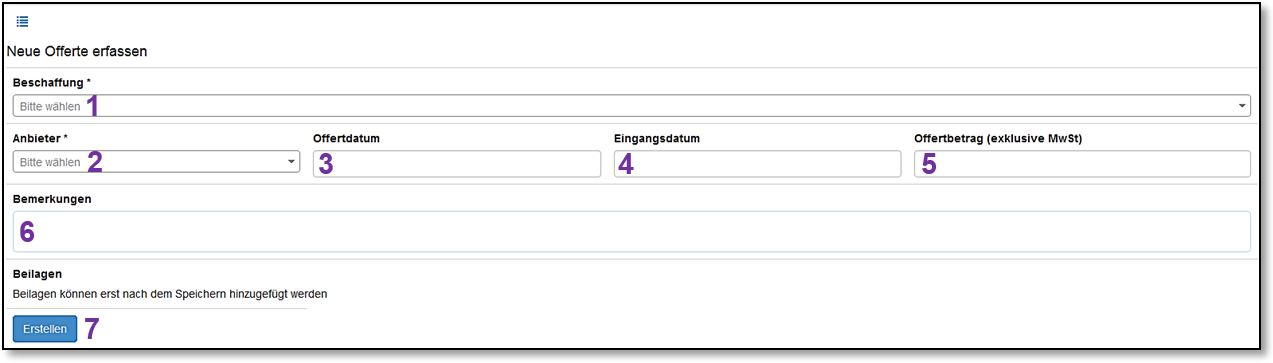
\includegraphics[width=1\linewidth]{715_OfferteErfassen.jpg}}
\caption{Adding a new tender}
% \label{fig:speciation}
\end{figure}


Mandatory fields are marked with an asterisk *. Fill out the fields:

\vspace{\baselineskip}

\begin{compactitem}
\item
Procurement \col{(1)}: From the drop-down menu, select the call for tender (procurement) to which the tender corresponds. Only calls for tender with the status 'Call for tender sent to invitees' appear.
\item
Tenderer \col{(2)}: Select the tenderer who sent the tender. If the call for tender was only sent to one invitee, only this invitee will appear in the drop-down menu.
\item
Date of tender \col{(3)}: Use the calendar selection to select the date stated on the tender.
\item
Date of receipt \col{(4)}: Use the calendar selection to select the date the tender was received.
\item
Amount \col{(5)}: Set the total sum of the tender. Only numbers and one point are accepted.
\item
Remarks \col{(6)}: You can enter free text in this field.
\end{compactitem}

\vspace{\baselineskip}

Click on the 'Create' button \col{(7)}. Afterwards, you can upload the 
tender:

\begin{figure}[H]
\center{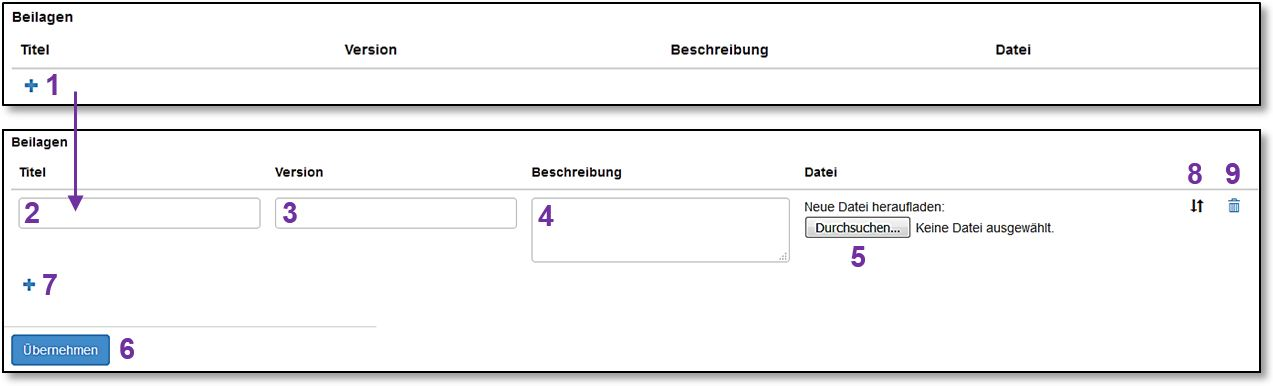
\includegraphics[width=1\linewidth]{715_OfferteHochladen.jpg}}
\caption{Uploading a tender}
% \label{fig:speciation}
\end{figure}

Click on the plus symbol 
\includegraphics[height=12pt]{/Icons/Pluszeichen.jpg} \col{(1)} to upload a tender. Enter the title \col{(2)}, and if need be the version number \col{(3)} and a description of the document \col{(4)} as free text in the corresponding fields. Click on 'Browse' \col{(5)} and select a file to upload it. If you have selected the wrong file, simply select a new file for upload. Click on 'Update' \col{(6)} to save.

\vspace{\baselineskip}

If the tender consists of multiple documents, click again on the plus symbol 
\includegraphics[height=12pt]{/Icons/Pluszeichen.jpg} \col{(7)} and repeat the procedure as many times as necessary. You can change the order of the documents by dragging and dropping the symbol with vertical arrows 
\includegraphics[height=12pt]{/Icons/VertPfeile.jpg} \col{(8)}. Click on the garbage bin symbol 
\includegraphics[height=12pt]{/Icons/Muelltonne.jpg} \col{(9)} to delete a document.

\vspace{\baselineskip}

\begin{wrapfigure}[7]{r}{6cm}
\vspace{-15pt}
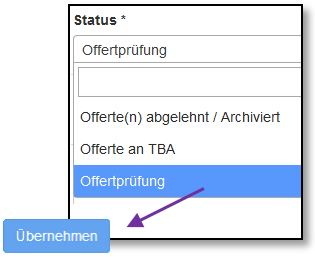
\includegraphics[height=50mm]{715_Offertpruefung.jpg}
% \caption{Status ändern}
\end{wrapfigure}
Go back to the list of procurements (menu on the left, menu item 'Procurement Function', sub-item 'Procurements') and open the procurement corresponding to the tender in edit mode by clicking on the pen symbol. Set the procurement status to 'Tender inspection'. Then click on 'Update'.

\vspace{\baselineskip}

\pagebreak
\subsubsection{Step 6: Establishing tender inspection logs and sending them to the decision-making body}

\begin{wrapfigure}[7]{r}{6cm}
  \vspace{-30pt}      % Grundwert war 20; mit 30 schön oben beim Text ausgerichtet
  \begin{center}
    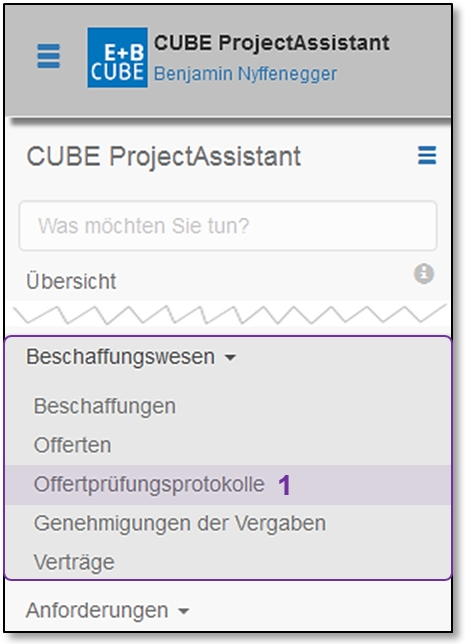
\includegraphics[height=80mm]{../chapters/07_Beschaffungswesen/pictures/7-1-6_Menu_Besch_Offertp.jpg}
  \end{center}
  \vspace{-20pt}
  \caption{Accessing the tender inspection logs}
  \vspace{-10pt}
\end{wrapfigure}

In the menu on the left, select the menu item 'Procurement Function' and the sub-item 'Tender Inspection Logs' \col{(1)}. The list of tender inspection logs appears.

\begin{center}
\hspace{-15pt}   
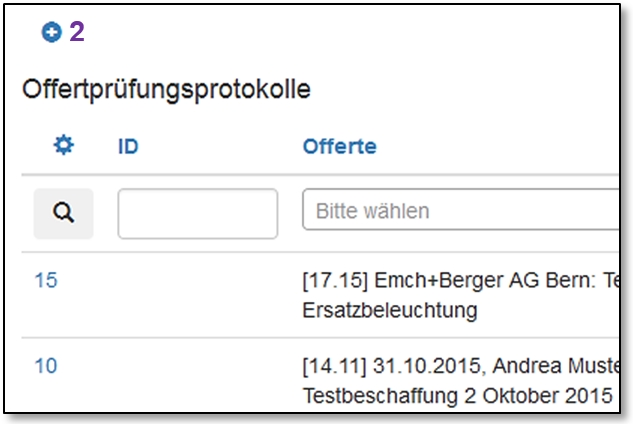
\includegraphics[width=.75\linewidth]{../chapters/07_Beschaffungswesen/pictures/7-1-6_NeuesOffertPruefProtokoll.jpg}
\end{center}

Click on the plus symbol 
\includegraphics[height=12pt]{/Icons/Plussymbol.jpg} \col{(2)} at the top left and the form for adding a new tender inspection log appears:

\begin{figure}[H]
\center{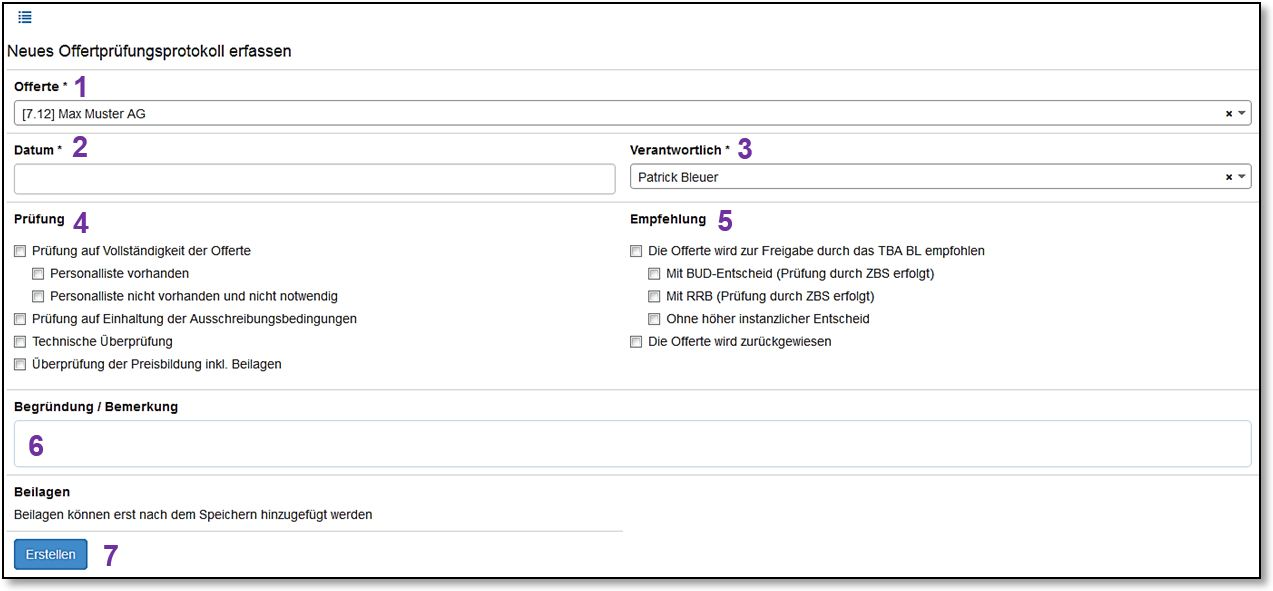
\includegraphics[width=1\linewidth]{716_OffertpruefungsprotokollErfassen.jpg}}
\caption{Adding a new tender inspection log}
% \label{fig:speciation}
\end{figure}

Mandatory fields are marked with an asterisk *. Fill out the fields:

\vspace{\baselineskip}

\begin{compactitem}
\item
In the top field, select the tender to be inspected. The selection list \col{(1)} only contains tenders for which no tender inspection log exists yet.
\item
\textcolor{black}{Date }\col{(2)} \textcolor{black}{: Use the calendar selection to set the date for the tender inspection log. }The current date is set by default.
\item
In the 'Responsible' field \col{(3)}, select the user responsible for the tender inspection log. The responsible is the user who will sign the tender inspection log.
\item {\sffamily
Under 'Check' \col{(4)} and 'Recommendation' \col{(5)} check the applicable boxes.}
\item
In the 'Justification/Remarks' field \col{(6)}, enter free text if needed.
\end{compactitem}

\vspace{\baselineskip}

Click on 'Create' \col{(7)}. Afterwards, attachments can be uploaded.

\begin{figure}[H]
\center{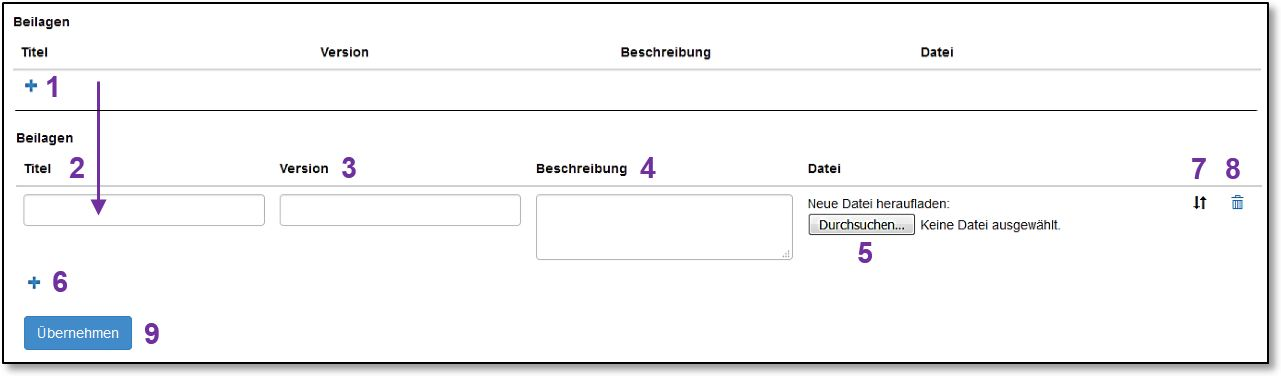
\includegraphics[width=1\linewidth]{716_OffertenpruefungsprotokollBeilagen.jpg}}
\caption{Uploading attachments to tender inspection logs}
% \label{fig:speciation}
\end{figure}

Click on the plus symbol 
\includegraphics[height=12pt]{/Icons/Pluszeichen.jpg} \col{(1)} to add an attachment. Enter the title \col{(2)}, and if needed the version \col{(3)} and a description of the document \col{(4)} as free text in the corresponding fields. Click 'Browse' \col{(5)} to select a file to be uploaded. If you have selected the wrong file, simply select a new one for upload. Click on 'Update' to save. \\
If multiple attachments are needed, click again on the plus symbol 
\includegraphics[height=12pt]{/Icons/Pluszeichen.jpg} \col{(6)} and repeat the procedure as many times as necessary. You can change the order of the documents by dragging and dropping the symbol with vertical arrows 
\includegraphics[height=12pt]{/Icons/VertPfeile.jpg} \col{(7)}. Click on the garbage bin symbol 
\includegraphics[height=12pt]{/Icons/Muelltonne.jpg} \col{(8)} to delete a document.

\vspace{\baselineskip}

\begin{wrapfigure}[7]{r}{5cm}
\vspace{-15pt}
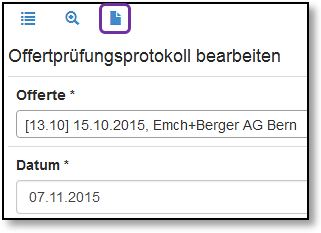
\includegraphics[height=40mm]{716_OffertpruefungsprotokollPDFgen.jpg}
% \caption{Status ändern}
\end{wrapfigure}
Click on 'Update' \col{(9)} to save the data. At the top left, 
click on the dog-eared paper symbol \includegraphics[height=12pt]{/Icons/BLattsymbol.jpg} to generate the tender inspection log as a PDF-file. Print out the tender inspection log and have it signed. The signed document should then be scanned and uploaded as an attachment to this tender inspection log. 
The original tender inspection log and the original tender should then be sent to the decision-making body.

\vspace{\baselineskip}

\begin{wrapfigure}[7]{r}{6cm}
\vspace{-15pt}
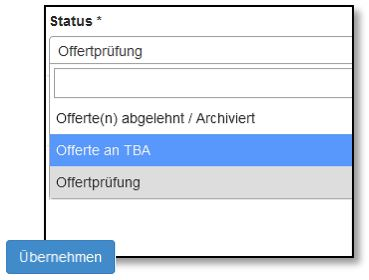
\includegraphics[height=50mm]{716_BeschaffungStatus.jpg}
% \caption{Status ändern}
\end{wrapfigure}
Go back to the list of procurements (menu on the left, menu item 'Procurement Function', sub-item 'Procurements') 
and open the procurement corresponding to the tender in edit mode by clicking on the pen symbol. Set the status to 'Tender with X'. Then click on 'Update'.

\vspace{\baselineskip}

Until the relevant body has issued the contract and had it signed by both parties, the process is put on hold in CUBE PA. Then, a copy of the contract should be added in CUBE PA to make its contents accessible.

\subsubsection{Step 7: Approval of the procedure by a position of higher order}

If, in the tender inspection log, you checked the box stating that the procedure is to be approved by a higher order (for example a government council), set the status to 'Decision position of higher order'.

\subsubsection{Step 8: Establishing a contract}

\begin{wrapfigure}[7]{r}{6cm}
  \vspace{-30pt}      % Grundwert war 20; mit 30 schön oben beim Text ausgerichtet
  \begin{center}
    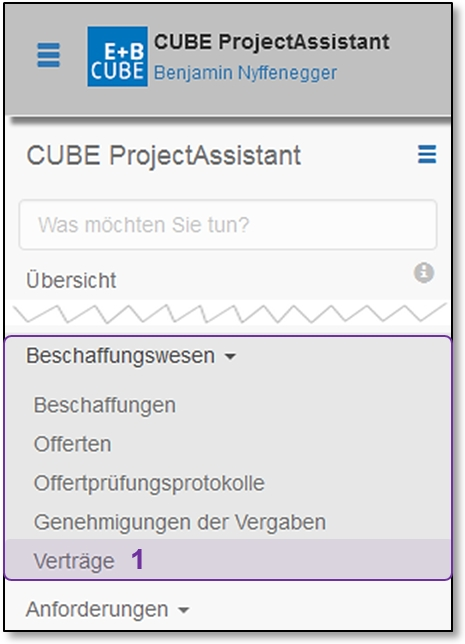
\includegraphics[height=80mm]{../chapters/07_Beschaffungswesen/pictures/7-1-8_Menu_Besch_Vertraege.jpg}
  \end{center}
  \vspace{-20pt}
  \caption{Accessing the contracts}
  \vspace{-10pt}
\end{wrapfigure}

Contracts are registered in TDCost (as basis for cost controlling) as well as in CUBE PA, to fully document the progress of the procurement and to make the contract contents accessible. When possibe, register the contract in TDCost first, so that you have access to all useful information 
from CUBE PA.

\begin{center}
\hspace{-55mm}   
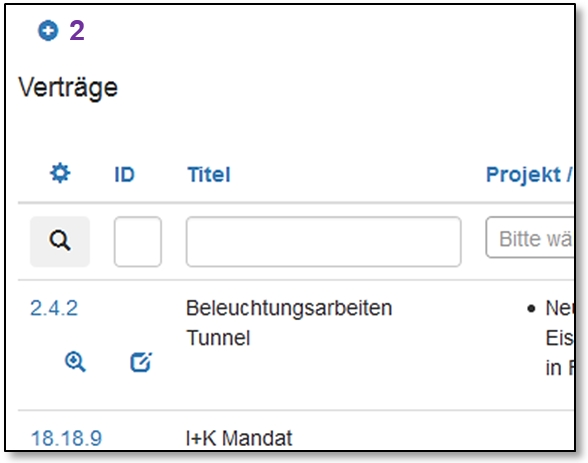
\includegraphics[width=.4\linewidth]{../chapters/07_Beschaffungswesen/pictures/7-1-8_NeuerVertrag.jpg}
\end{center}

\vspace{\baselineskip}

In the menu on the left, select the menu item 'Procurement Function' and the sub-item 'Contracts' \col{(1)}. The list of contracts appears.

\vspace{\baselineskip}

Click on the plus symbol 
\includegraphics[height=12pt]{/Icons/Plussymbol.jpg} \col{(2)} at the top left and the form for adding a new contract appears. The list symbol \includegraphics[height=12pt]{/Icons/Listensymbol_zurueck.jpg} \col{(3)} takes you back to the list / overview.

\begin{figure}[H]
\center{\includegraphics[width=1\linewidth]{718_VertragErfassen.jpg}}
\caption{Adding a new contract}
% \label{fig:speciation}
\end{figure}

Mandatory fields are marked with an asterisk *. Fill out the fields:

\vspace{\baselineskip}

\begin{compactitem}
\item {\sffamily\color{black}
Under 'Tender', select the tender that served as a basis for this contract. Only tenders belonging to an ongoing procurement are listed in the drop-down menu.}
\item
The 'Contract title' is automatically set based on the tender information, but you can still edit it.
\item
The 'Project/Subproject' is also automatically set based on the tender information, but you can still change the selection.
\item
The 'Contract date' can be set with the calendar selection.
\item
The 'Start date' and the 'End date' are also set with a calendar selection. These are the dates on which the service provision should start and end.
\item
The 'Client' can be selected from a drop-down list and 'Contractor' is set automatically based on the tender information.
\item
The 'Contract sum' is also set automatically based on the tender information. You can still change the sum, for example if only a part of the offered services are included in the contract.
\item
The 'External Reference (Contract)' (free text field) and 'External status' (drop-down list) refer to the classification of the contract by other systems (for example TDCost). If the contract is not listed in another system, set the status to 'undefined'.
\item
Under 'Controller', select the person responsible for supervising the contract, and right next it select their replacement.
\item
The field 'Content' contains automatically information from the tender that you can modify, for example if only a part of the offered services are included in the contract.
\item
In the 'Remarks' field, you can enter free text.
\end{compactitem}

\vspace{\baselineskip}

Click on 'Create' \col{(4)} and afterwards you can upload the contract.

\begin{figure}[H]
\center{\includegraphics[width=1\linewidth]{718_VertragHochladen.jpg}}
\caption{Uploading a contract}
% \label{fig:speciation}
\end{figure}

Click on the plus symbol \includegraphics[height=12pt]{/Icons/Pluszeichen.jpg} \col{(1)} to upload a contract. Enter the title \col{(2)}, and if needed the version \col{(3)} and a description of the document \col{(4)} as free text in the corresponding fields. Click on 'Browse' \col{(5)} to select a file for upload. If you have selected the wrong file, simply select a new one for upload . Click on 'Update' \col{(6)} to save the data.

\vspace{\baselineskip}

If the contract consists of multiple documents, click again on the plus symbol \includegraphics[height=12pt]{/Icons/Pluszeichen.jpg} \col{(7)} and repeat the procedure as many times as necessary. You can change the order of the documents by dragging and dropping the symbol with vertical arrows \includegraphics[height=12pt]{/Icons/VertPfeile.jpg} \col{(8)}. Click on the garbage bin symbol \includegraphics[height=12pt]{/Icons/Muelltonne.jpg} \col{(9)} to delete a document.

\vspace{\baselineskip}

Go back to the list of procurements (menu on the left, menu item 'Procurement Function', sub-item 'Procurements') and open the procurement corresponding to the contract in edit mode by clicking on the pen symbol. Set the status to 'Procurement completed'. Then click on 'Update'.

\vspace{\baselineskip}

\textbf{Adding an additional contract to an existing tender.}

If you need to add an additional contract to a tender for which a contract has already been added, for example because another partial service is to be provided, first look for procurement in question in the procurements list, and if the status is set to 'Procurement completed', change it to 'Signature X / Dispatch'. This ensures that the tender can be selected when the contract is added. Once you have added the new contract, set the status back to 'Procurement Completed'.

\subsubsection{Handling a tender for which there was no call for tender}

It may happen that you have to add a tender for which no call for tender has been sent. For example, it was agreed at a meeting that someone would submit a tender, or that someone would submit an addendum to an existing contract. In such cases, proceed as follows:

\begin{itemize}
\item
Initialise a procurement, as described in step 2, without entering any information that has to do with sending a call for tender. If the tender is a follow-up tender, select the tender for which this new tender represents an addendum in the 'Supplementary budget for procurement' field.
\item
Skip steps 3 and 4.
\item
Add the tender as described in step 5. This step and the following steps work exactly the same way as for an offer made on the basis of a call for tender.
\end{itemize}

\subsection{Workflow for procurements by invitation procedure or open procedure}

An example workflow for procurements by invitation or open procedure will follow later.
